
\section{Time Dependent discontinuity problem}
\label{section:time_problem}
In the time dependent disconinuity problem, we change the value of the parameter $\beta$ from 0.9 to 0.005 at time 27. This introduces a discontinuity in the problem. We will show that this leads to inaccuracies, especially with fixed step solvers. We then introduce a form of discontinuity handling using cold starts to show an efficient way to solve time dependent discontinuity problems.

\subsection{Naive treatment of Covid-19 time discontinuity models}
\label{subsection:naive_time_problem}
A naive implementation of the problem is to use an if-statement inside the right hand side function, $f(t, y)$, to implement the changes in $\beta$ as measures are implemented. An if-statement makes the function f(t, y) and its derivatives discontinuous. This introduces problems as outlined in Section $\ref{subsection:effect_of_discontinuity}$.

For this report, we will add a time-dependent discontinuity by using an if statement at time 27, where the parameter $\beta$ will change from 0.9 to 0.005, indicating that measures are implemented. In pseudo code, this looks like:

\begin{minipage}{\linewidth}
\begin{lstlisting}[language=Python]
function model_with_if(t, y)
    (S, E, I, R) = y
    beta = 0.005
    if t < 27:
        beta = 0.9
           	
    // code to get (dSdt, dEdt, dIdt, dRdt)
    return (dSdt, dEdt, dIdt, dRdt)
\end{lstlisting}
\end{minipage}

Also, to stay true to a naive treatment, we will always use the default tolerances in this section. Discrepancies across the programming environments that can be due to tolerance issues are investigate in Section $\ref{subsection:time_tolerance_study}$.
 
\subsubsection{Time discontinuity in R}
\begin{figure}[h]
	\centering
	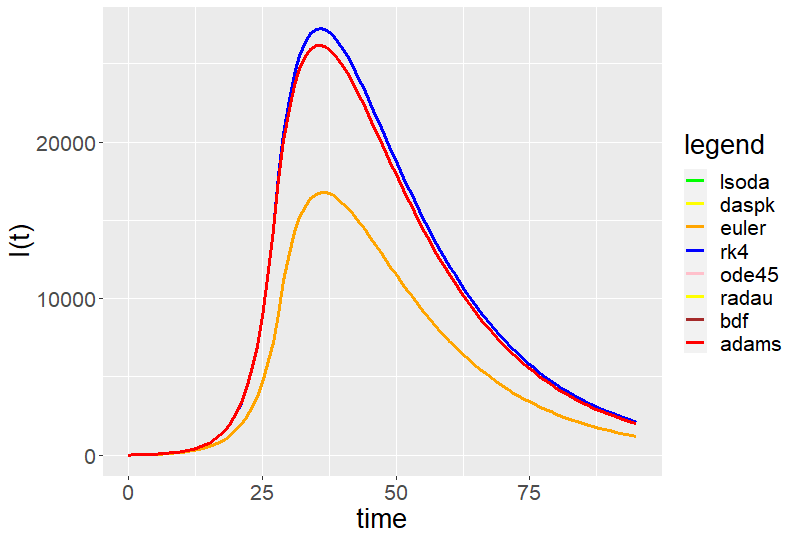
\includegraphics[width=0.7\linewidth]{./figures/time_discontinuity_R}
	\caption{Time Discontinuity in R}
	\label{fig:time_discontinuity_R}
\end{figure}
From Figure $\ref{fig:time_discontinuity_R}$, we can see that all the methods except 'euler' and 'rk4' are on the same line. 'rk4' is somehow close to the actual solution but 'euler' was completely wrong. We note that all the other methods had error control while these two are fixed step-size solvers.

We also note that 'rk4' is doing better than 'euler' for this specific problem as it has a higher order. But the way it is performing is still better than expected. We prove in another experiment that this is entirely because of the outputting problem discussed in Section $\ref{subsection:solution_output_points_impl}$. In fact, if we use a bigger step-size, 'rk4' gives results which are as bad as 'euler'. Figure $\ref{fig:rk4_messing_up_no_event_R}$ shows that experiment with 'rk4' at different initial step-size (space between the output points) plotted against a graphically accurate solution in red. We can see that as soon as we change the step-size for 'rk4', it does not give good results at all. Analysing the source for 'rk4' and 'euler' shows that it picks the step size using the output points requested. Spacing out the output points affect the step-size which affects the accuracy of the fixed step-size solver.

A solution to this problem of wanting to use 'rk4', 'euler' or any user-programmed solver would be to have a small initial step-size but we cannot know beforehand how small is small enough. A better solution would be to not use fixed-step size solvers, be it from the packages or user-implemented ones. Reputable methods with error control should be preferred as we have shown that these solvers can step over one discontinuity by resizing the step repeatedly, as we have seen is needed in Section $\ref{subsection:effect_of_discontinuity}$.

\begin{figure}[h]
	\centering
	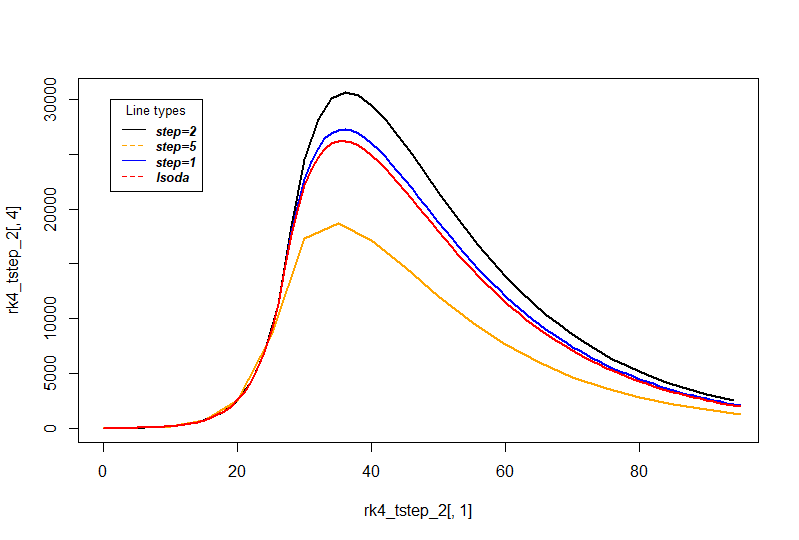
\includegraphics[width=0.7\linewidth]{./figures/rk4_messing_up_no_event_R}
	\caption{R's rk4 with bigger step-size}
	\label{fig:rk4_messing_up_no_event_R}
\end{figure}


\subsubsection{Time discontinuity in Python}
\begin{figure}[h]
	\centering
	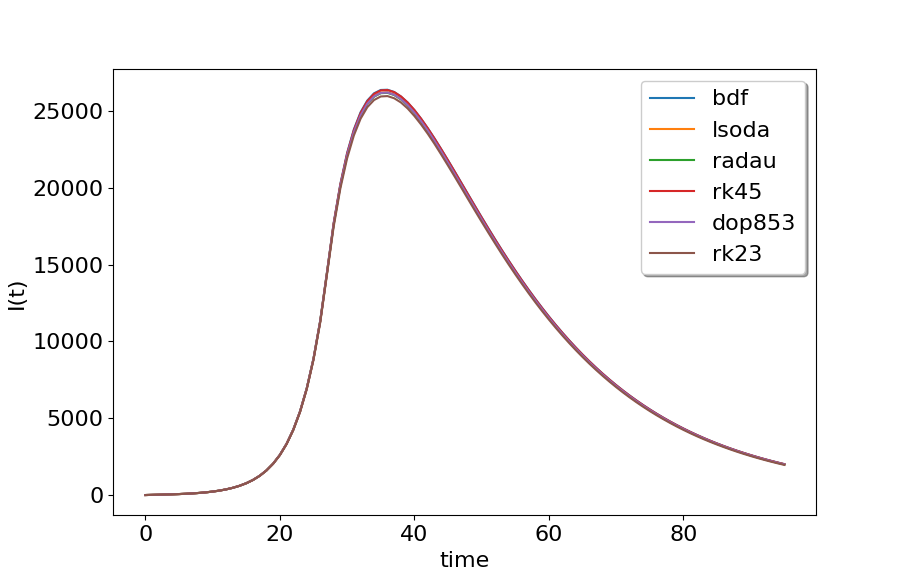
\includegraphics[width=0.7\linewidth]{./figures/time_discontinuity_py}
	\caption{Time Discontinuity in Python}
	\label{fig:time_discontinuity_py}
\end{figure}
From Figure $\ref{fig:time_discontinuity_py}$, we can see that all the methods in Python's $solve\_ivp()$ work correctly. There is some blurring at the peak but all the methods are along the same line. Python only provides error-controlled packages and thus we can see that error-control is all that is needed to step over one discontinuity. This observation also leads us to another conclusion that sharp tolerance with an error-control solution is what is required to step over one discontinuity.

\subsubsection{Time discontinuity in Scilab}
\begin{figure}[h]
	\centering
	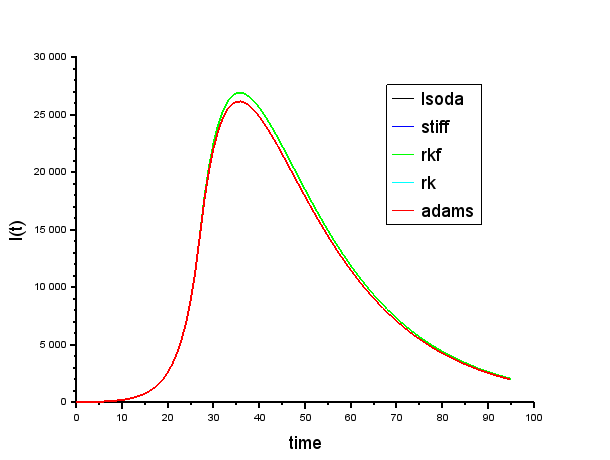
\includegraphics[width=0.7\linewidth]{./figures/time_discontinuity_scilab}
	\caption{Time Discontinuity in Scilab}
	\label{fig:time_discontinuity_scilab}
\end{figure}
From Figure $\ref{fig:time_discontinuity_scilab}$, in Scilab, all the methods are on the same line except for 'rkf'. This is more interesting as we know that 'rkf' should also have error control. This is explained by noting that 'rkf' has smaller default absolute and relative tolerances in Scilab. We will show during a tolerance analysis in Section $\ref{subsection:time_tolerance_study}$ that with a sharp enough tolerance, it also provides the right solution.

The other methods are all error-controlled and are on the same line as expected. We note that all of the other methods have a higher default tolerance than 'rkf' and thus this result is not surprising.

This also points to us that an error control solver with a sharp tolerance is able to step over a discontinuity.
  

\subsection{Better way to treat discontinuities in the time models}
\label{subsection:time_disc_handling}
A better way to solve the time dependent discontinuity problem is to make use of cold starts so that we integrate before and after the discontinuity with different (separate) calls to the solver. Cold starting at a time dependent discontinuity improves the accuracy as we will see in this and the next section. It also improves the efficiency as less function calls are required since we do not have the spike in function calls due to repeated step-size resizing described in Section $\ref{subsection:effect_of_discontinuity}$.

A cold start will entail using new unfilled data structures with no values from previous computations corrupting the new integration. It will also use new initial step sizes and for methods of varying order like the BDF and Adams, we start anew with the default order.  Each call thus do not overlap and the solver thus integrates a continuous subinterval with each call and will not have to step over a discontinuity.

To solve the time discontinuity problem, we will integrate from time 0 to the time that measures are implemented, 27, with one call to the solver and use its solution values at time 27 as the initial values to make another call that will integrate from then to the end. The pseudo-code is as follows:

\begin{minipage}{\linewidth}
\begin{lstlisting}[language=Python]
initial_values = (S0, E0, I0, R0)
tspan_before = [0, 27]
solution_before = ode(intial_values, model_before_measures,
 tspan_before)

initial_values_after = extract_last_row(solution_before)
tspan_after = [27, 95]
solution_after = ode(intial_values_after, 
model_after_measures, tspan_after)

solution = concatenate(solution_before, solution_after)
\end{lstlisting}
\end{minipage}

This technique can be applied by epidemiologists for any problem where they know when the discontinuity is introduced or any time they feel that a time dependent if-statement should be added to their model.

 \subsubsection{Solving time discontinuity in R} 
\begin{figure}[h]
	\centering
	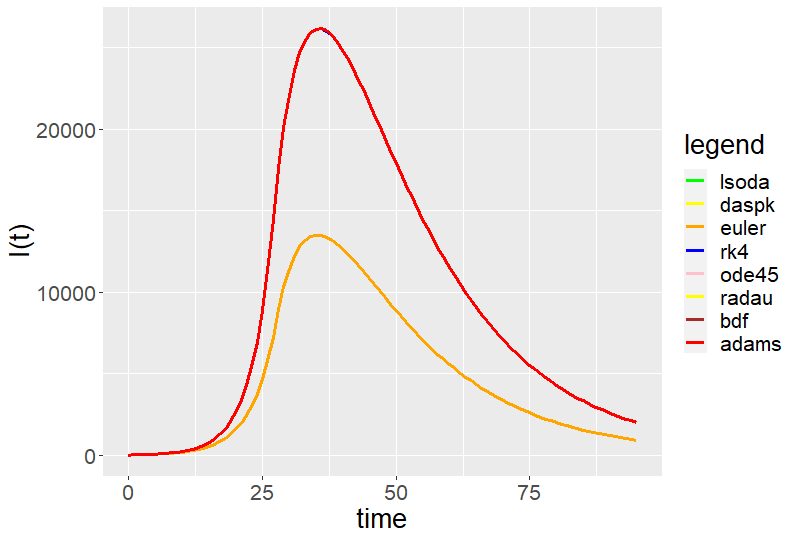
\includegraphics[width=0.7\linewidth]{./figures/solve_time_discontinuity_R}
	\caption{Solving Time Discontinuity in R}
	\label{fig:solve_time_discontinuity_R}
\end{figure}
From Figure $\ref{fig:solve_time_discontinuity_R}$, the 'euler' method still fails even with the discontinuity handling. This is as expected as it has no error control and thus it still suffers from the stability issues and will require smaller steps to integrate even continuous problems.

We see that breaking the problem into two makes 'rk4' perform better. The method has a higher order, meaning that it does not need as small an initial step size as 'euler' to solve the two continuous problems but this exceptionally well performance is still unexpected. We will show in Figure $\ref{fig:rk4_messing_up_with_event_R}$ that this is only due to a very small initial step size and the problem with the old method of outputting points as described in Section $\ref{subsection:solution_output_points_impl}$.

\begin{figure}[h]
	\centering
	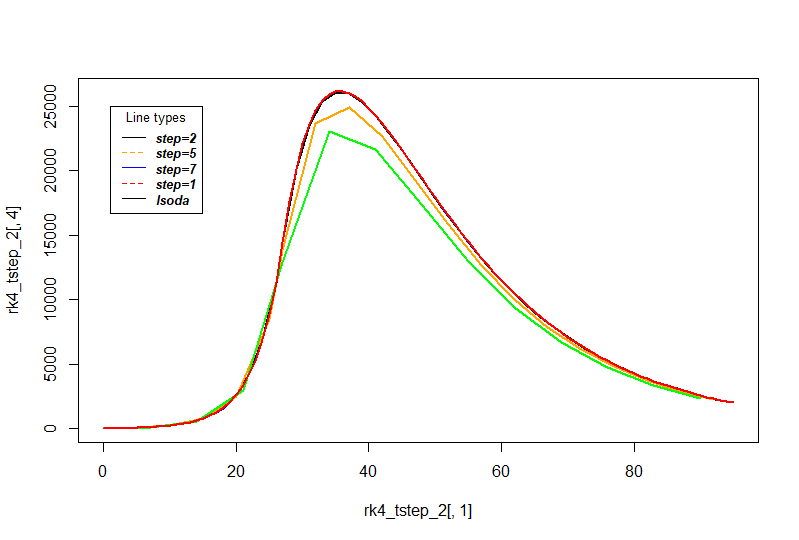
\includegraphics[width=0.7\linewidth]{./figures/rk4_messing_up_with_event_R}
	\caption{R's rk4 with bigger step-size with discontinuity handling}
	\label{fig:rk4_messing_up_with_event_R}
\end{figure}

Thus our recommendation to avoid fixed step size solvers still holds as for any particular problem, researchers will never know how small the step size should be without knowing the actual solution.

We also note again, that all the error-controlled solvers perform well. We will see, from the efficiency data, that using cold starts is more efficient. Using cold starts, the error control solvers do not have to step over a discontinuity and we will not have the rise in the number of function evaluation as we discussed in $\ref{subsection:effect_of_discontinuity}$. Table $\ref{tab:time_discontinuity_R}$ shows that discontinuity handling reduces the number of function evaluations. 

\begin{table}[h]
\caption {R Time Discontinuity problem efficiency data} \label{tab:time_discontinuity_R}
\begin{center}
\begin{tabular}{ c c c } 
 method & nfev & event's nfev \\ 
euler & 96  & 97  \\
rk4   & 381 & 382 \\ 
lsoda & 332 & 272 \\
ode45 & 735 & 599 \\
radau & 679 & 585 \\
bdf   & 423 & 263 \\
adams & 210 & 176 \\
daspk & 517 & 521
\end{tabular}
\end{center}
\end{table}

Our analysis of the efficiency data in Table $\ref{tab:time_discontinuity_R}$ starts by noting that the non-error controlled solvers in the 'euler' and 'rk4' methods have the same number of function evaluations, the additional one being due to integrating twice at time 27. This indicates that they are just stepping from output point to output point using the same fixed step-size both with and without the discontinuity handling.

Next, we note the drastic decreases in the number of function evaluations from all the remaining solvers except 'daspk'. These reductions in the number of function evaluations will have a significant impact on the CPU time if the problem were harder. This is entirely explained in $\ref{subsection:effect_of_discontinuity}$ where the error controlled solvers have to repeatedly resize the step-size as they encounter a discontinuity. Not having to integrate through a discontinuity means that there is no need to perform the 'crash' into a discontinuity.

VI =======================
Finally, we explain the almost constant value of dapsk's number of function evaluations through the fact that it may have some inherent discontinuity handling and thus even without the treatment we did, it could still detect discontinuity and integrate as usual. IT COULD ALSO BE BECAUSE daspk DEPENDS ON THE SPACING BETWEEN THE POINTS.
======================== VI

In Section $\ref{subsection:time_tolerance_study}$, we will see that this discontinuity handling also allows us to use coarser tolerances.

\subsubsection{Solving time discontinuity in Python} 
\begin{figure}[h]
	\centering
	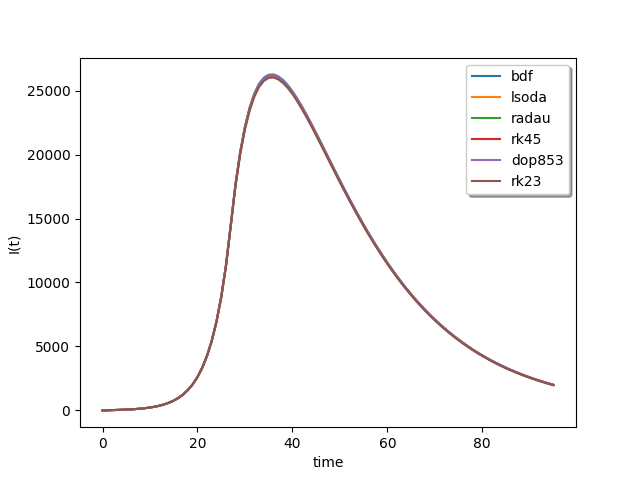
\includegraphics[width=0.7\linewidth]{./figures/solve_time_discontinuity_py}
	\caption{Solving Time Discontinuity in Python}
	\label{fig:solve_time_discontinuity_py}
\end{figure}
Python did not have a problem even with the if-statement inside. This is because all the available methods use error control in Python and its default tolerances were sharp enough. From Figure $\ref{fig:solve_time_discontinuity_py}$, we can see that Python again gave the correct results. Furthermore, the slight blurring at the peak has disappeared. The addition of discontinuity handling will also drastically reduce the number of function evaluations as seen in Table $\ref{tab:time_discontinuity_Py}$.

\begin{table}[h]
\caption {Python Time Discontinuity problem efficiency data} \label{tab:time_discontinuity_Py} 
\begin{center}
\begin{tabular}{ c c c }
 method & nfev & event nfev \\ 
lsoda  & 162 & 124 \\
rk45   & 134 & 130 \\
bdf    & 202 & 146 \\
radau  & 336 & 220 \\
dop853 & 329 & 181 \\
rk23   & 152 & 127 \\
\end{tabular}
\end{center}
\end{table}

VI =========================
LOOKING THROUGH MY OLD CODE, I AM NOT USING PYTHON's INTERPOLATION MODE to get the above data. I am using the $t\_eval$ mode.... 
I AM WORKING ON REWRITING ALL MY OLD PYTHON CODE TO USE interpolation
======================= VI

From Table $\ref{tab:time_discontinuity_Py}$, we see that across the board, the methods take less function evaluations. There are some huge changes for 'BDF', 'DOP853' and 'Radau'. There are slight decreases in 'LSODA' and 'RK23' and only a very small decrease in 'RK45'. In Section $\ref{subsection:time_tolerance_study}$, we will see that this discontinuity handling also allows us to use coarser tolerances.

\subsubsection{Solving time discontinuity in Scilab} 
\begin{figure}[h]
	\centering
	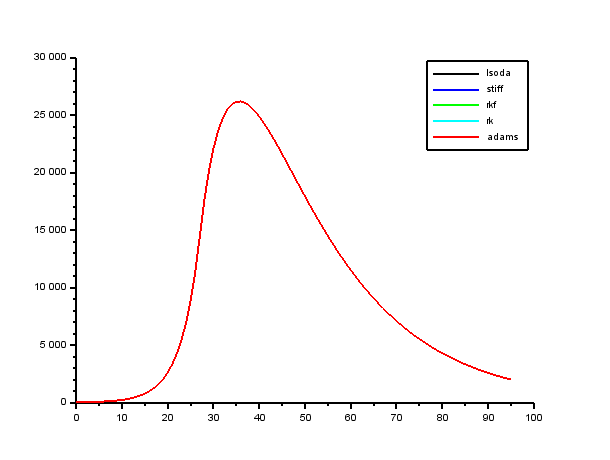
\includegraphics[width=0.7\linewidth]{./figures/solve_time_discontinuity_scilab}
	\caption{Solving Time Discontinuity in Scilab}
	\label{fig:solve_time_discontinuity_scilab}
\end{figure}
We can see from Figure $\ref{fig:solve_time_discontinuity_scilab}$ that all the methods lie on a single line and thus the time discontinuity has been solved. The 'rkf' method is also on that line and is correctly solving the solver. This is despite the fact that 'rkf' has a coarser default tolerance. In Section $\ref{subsection:time_tolerance_study}$, we will see that this discontinuity handling also allows us to use coarser tolerances and thus explains why the default tolerance 'rkf' is also solving the problem correctly.

The addition of discontinuity handling will also drastically reduce the number of function evaluations as seen in Table $\ref{tab:time_discontinuity_scilab}$.

\begin{table}[h]
\caption {Scilab Time Discontinuity problem efficiency data} 
    \label{tab:time_discontinuity_scilab} 
\begin{center}
\begin{tabular}{ c c c }
 method & nfev & event nfev \\ 
    lsoda & 346  & 292 \\
    stiff & 531  & 362 \\
    rkf   & 589  & 590 \\
    rk    & 1649 & 1473 \\
    adams & 304  & 221  \\
\end{tabular}
\end{center}
\end{table}

From Table $\ref{tab:time_discontinuity_sci}$, we see that across the board, the methods take less function evaluations. We see substantial decreases in the number of function evaluations for lsoda, stiff, rk and adams.

The odd values of 'rkf' whereby the number of function evaluations does not decrease is because 'rkf' is using the old method for outputting points as outlined in Section $\ref{subsection:solution_output_points_impl}$.

VI =========================
FORTRAN's rkf DOES NOT USE INTERPOLATION!!!!!

MIGHT NEED TO ADD ANOTHER STUDY in Scilab WHERE we space out the points more.

I think some of its other methods ALSO DON'T
========================== VI

\subsection{Efficiency data and tolerance study for the time discontinuous problem}
\label{subsection:time_tolerance_study}
It is not uncommon for researchers to use the ODE in a loop or within an optimisation algorithm so that they can get models with different parameters. In so doing, some may be tempted to coarsen the tolerances whenever the experiment they are performing is taking too long. In this Section, we investigate how coarse we can set the tolerance while keeping accurate results. 

We investigate 'lsoda' across R, Python and Scilab as they all appear to use the same source code. We use this experiment to show that the discontinuity handling allow us to use coarser tolerances.

We will also investigate 'rkf' in Scilab as it has a smaller default tolerance and will prove that it can solve the problem without discontinuity handling only for sharper tolerances than its default. We also investigate Runge-Kutta pairs of the same order in the other programming environments. R and Python have a version of DOPRI5 but do not share the same source code, the DOPRI5 in Python being a Python implementation and the one in R being a Fortran implementation. We also note that R is not using DOPRI5.f but another Fortran implementation of DOPRI5.

\subsubsection{Comparing LSODA across platforms for time discontinuous problem}

In this Section, we run R's LSODA solver with multiple tolerances with and without discontinuity handling. We will set both the relative and absolute tolerances to particular values and see how coarse we can keep the tolerance while still having accurate results. We also look at efficiency data to see the decreases in the number of function evaluations, which would lead to significant decreases in computation times.

\subparagraph{Time discontinuity LSODA tolerance study in R}
\begin{figure}[h]
	\centering
	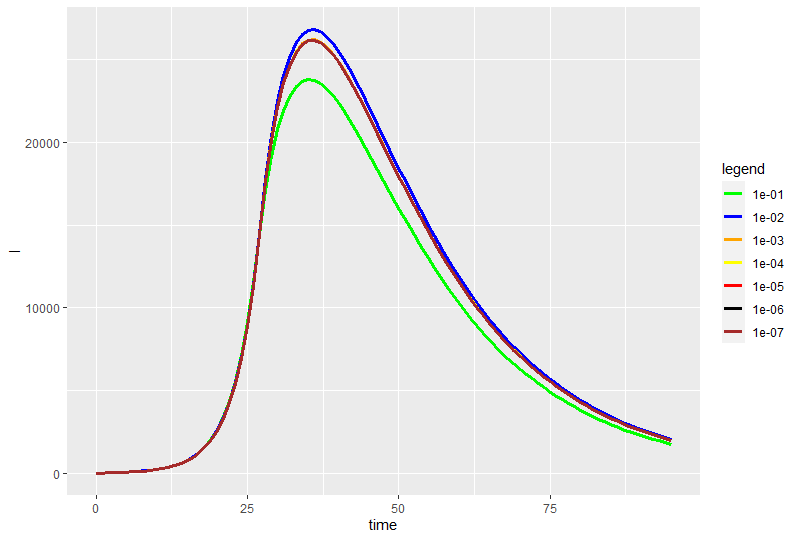
\includegraphics[width=0.7\linewidth]{./figures/tolerance_time_lsoda_no_event_R}
	\caption{Time discontinuity tolerance study on R's LSODA without a cold start}
	\label{fig:tolerance_time_lsoda_no_event_R}
\end{figure}

\begin{figure}[h]
	\centering
	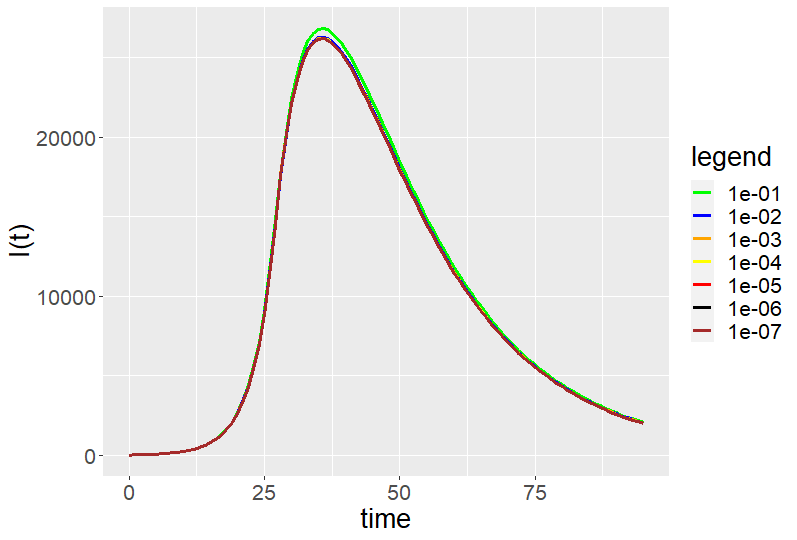
\includegraphics[width=0.7\linewidth]{./figures/tolerance_time_lsoda_with_event_R}
	\caption{Time discontinuity tolerance study on R's LSODA with a cold start}
	\label{fig:tolerance_time_lsoda_with_event_R}
\end{figure}

From Figures $\ref{fig:tolerance_time_lsoda_no_event_R}$ and $\ref{fig:tolerance_time_lsoda_with_event_R}$, we can see that the addition of discontinuity handling lets us use a coarser tolerance and still get the required answer; we need $10^{-3}$ and sharper tolerances without discontinuity handling but can use $10^{-2}$ and sharper with it. This solidifies that a form of discontinuity handling when coding a discontinuous problem will improve the accuracy of the solution. Also, using coarser tolerances gives us more efficiency, as we will see in Table $\ref{tab:tolerance_time_discontinuity_lsoda_R}$. This allows researchers to coarsen the tolerances of their experiment when the latter is running too slow.

\begin{table}[h]
\caption {R LSODA Time Discontinuity tolerance study} \label{tab:tolerance_time_discontinuity_lsoda_R} 
\begin{center}
\begin{tabular}{ c c c c c }
tolerance & nfev & nsteps & event nfev & event nsteps \\ 
1e-01 & 197 &  98 & 200 &  99 \\
1e-02 & 214 & 104 & 206 & 101 \\
1e-03 & 264 & 122 & 212 & 105 \\
1e-04 & 264 & 123 & 224 & 111 \\
1e-05 & 317 & 145 & 244 & 121 \\
1e-06 & 332 & 154 & 272 & 133 \\
1e-07 & 393 & 185 & 298 & 146 \\
\end{tabular}
\end{center}
\end{table}

From Table $\ref{tab:tolerance_time_discontinuity_lsoda_R}$, we see that for the coarser tolerances, the number of function evaluations is roughly the same. But with sharper tolerances, a lot more function evaluations are required and thus if we had a user-provided function which took longer to run, we will see clear drops in computation times.

The similar number of function evaluations for the coarser tolerances should not distract from the fact that the code without discontinuity at these tolerances are not as accurate as the code with. The small differences of 3 function evaluations for the 0.1 tolerance case and 8 function evaluations in the 0.01 case do not excuse that the solutions are wrong.

\subparagraph{Time discontinuity LSODA tolerance study in Python}
In this Section, we run Python's LSODA solver with multiple tolerances with and without discontinuity handling. We note that Python was working correctly in both cases apart from some blurring but we will see how coarse we can keep the tolerance while still having correct results. We set both the relative and absolute tolerances to particular values. We also look at efficiency data to see the decreases in the number of function evaluations.

\begin{figure}[h]
	\centering
	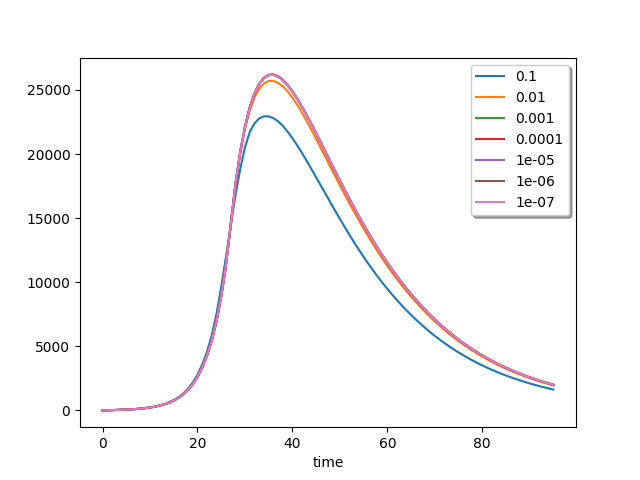
\includegraphics[width=0.7\linewidth]{./figures/tolerance_time_lsoda_no_event_py}
	\caption{Time discontinuity tolerance study on Python's LSODA without a cold start}
	\label{fig:tolerance_time_lsoda_no_event_py}
\end{figure}

\begin{figure}[h]
	\centering
	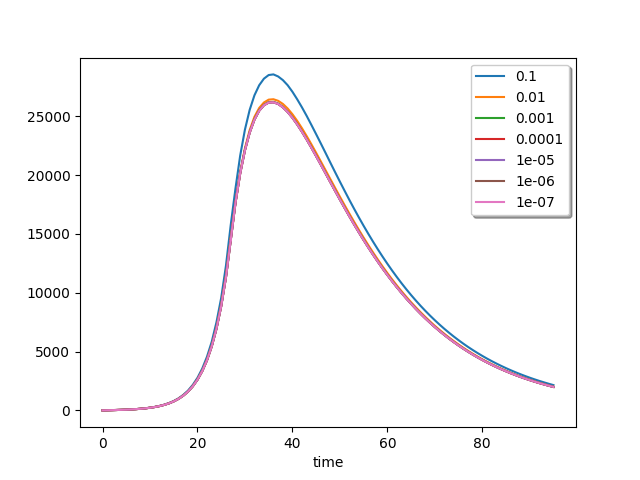
\includegraphics[width=0.7\linewidth]{./figures/tolerance_time_lsoda_with_event_py}
	\caption{Time discontinuity tolerance study on Python's LSODA with a cold start}
	\label{fig:tolerance_time_lsoda_with_event_py}
\end{figure}

From Figures $\ref{fig:tolerance_time_lsoda_with_event_py}$ and $\ref{fig:tolerance_time_lsoda_no_event_py}$, the addition of the discontinuity handling lets us use a coarser tolerance, as $10^{-2}$ was enough to get the correct answer with the discontinuity handling whereas $10^{-3}$ was needed without. This essentially tells us that using discontinuity handling will improve our results for a more complex time-dependent discontinuity problem.

In turn, the use of coarser tolerances give us more efficiency. (See Table $\ref{tab:tolerance_time_discontinuity_lsoda_py}$.)

We also note that the results using LSODA in Python and R are very similar which stems from the fact that they are using the same source code.

\begin{table}[h]
\caption {Python LSODA Time Discontinuity tolerance study} \label{tab:tolerance_time_discontinuity_lsoda_py} 
\begin{center}
\begin{tabular}{ c c c }
tolerance & nfev  & event nfev \\ 
0.1    & 79.0  & 86.0  \\
0.01   & 98.0  & 93.0  \\
0.001  & 156.0 & 116.0 \\
0.0001 & 185.0 & 146.0 \\
1e-05  & 259.0 & 186.0 \\
1e-06  & 283.0 & 228.0 \\
1e-07  & 361.0 & 272.0 \\
\end{tabular}
\end{center}
\end{table}
Again, in Table $\ref{tab:tolerance_time_discontinuity_lsoda_py}$, we see that that at coarse tolerances, the number of function evaluations is roughly the same. This similar number of function evaluations does not excuse the fact that the coarser tolerances are giving erroneous values. 

At sharp tolerance, where the comparison is fair, the number of function evaluations is much smaller with the discontinuity handling than without; we make 40 less function evaluations at 0.001 and 0.0001 but we do much less function evaluations for sharper tolerances. We note that if the user-provided function was more time-consuming, this reduced number of function evaluations will cause a decrease in the CPU times. This reduced number of function evaluations stems from the facts discussed in Section $\ref{subsection:effect_of_discontinuity}$. 

\subparagraph{Time discontinuity LSODA tolerance study in Scilab}
In this Section, we run Scilab's LSODA solver with multiple tolerances with and without discontinuity handling. We will set both the relative and absolute tolerances to particular values and see how coarse we can keep the tolerance while still getting correct results.

\begin{figure}[h]
	\centering
	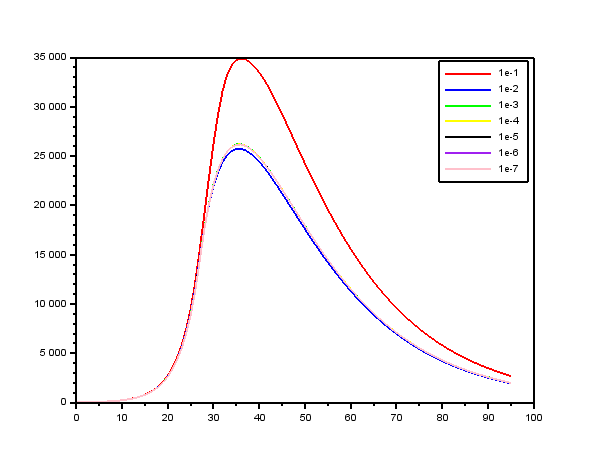
\includegraphics[width=0.7\linewidth]{./figures/tolerance_time_lsoda_no_event_sci}
	\caption{Time discontinuity tolerance study on Scilab's lsoda without a cold start}
	\label{fig:tolerance_time_lsoda_no_event_sci}
\end{figure}

\begin{figure}[h]
	\centering
	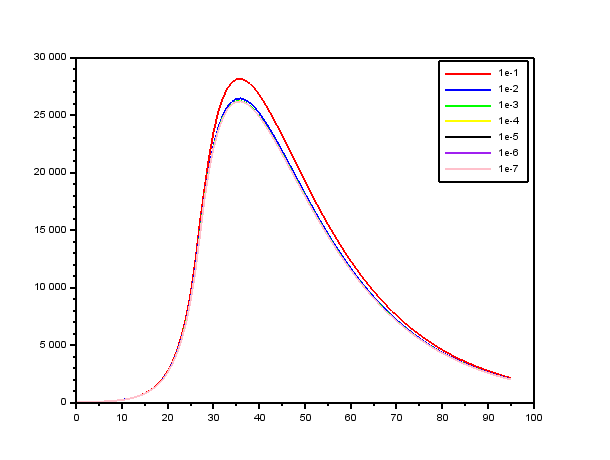
\includegraphics[width=0.7\linewidth]{./figures/tolerance_time_lsoda_with_event_sci}
	\caption{Time discontinuity tolerance study on Scilab's lsoda with a cold start}
	\label{fig:tolerance_time_lsoda_with_event_sci}
\end{figure}

From Figures $\ref{fig:tolerance_time_lsoda_no_event_sci}$ and $\ref{fig:tolerance_time_lsoda_with_event_sci}$ we can see that at $10^{-1}$ to $10^{-4}$, Scilab's LSODA without discontinuity handling fails but we seem to be able to use $10^{-3}$ with the discontinuity handling. 

It is interesting to see how far off the solution without discontinuity handling is at a tolerance of $10^{-1}$. We also note that this behaviour is different from R's and Python's LSODA 

VI ===================== 
but this may be due to the way Scilab processes the tolerances before haning it to the source code
==================== VI

\begin{table}[h]
\caption {Scilab LSODA Time Discontinuity tolerance study} 
    \label{tab:tolerance_time_discontinuity_lsoda_scilab} 
\begin{center}
\begin{tabular}{ c c c }
tolerance & nfev & event nfev \\ 
    0.1   & 80.  & 82.   \\
    0.01  & 98.  & 92.   \\
    0.001 & 156. & 116.  \\
    1e-4  & 185. & 146.  \\
    1e-5  & 255. & 186.  \\
    1e-6  & 280. & 228.  \\
    1e-7  & 361. & 272.  \\
\end{tabular}
\end{center}
\end{table}
Again, in Table $\ref{tab:tolerance_time_discontinuity_lsoda_scilab}$, we see that the number of function evaluations is roughly the same at coarser tolerances but that at sharp tolerances, where both give accurate solution and thus allow far comparison, the code with the discontinuity handling performs better than the code without. We can use up to 90 less function evaluations through discontinuity handling.  

\subsubsection{Comparing Runge-Kutta pairs across platforms for the time discontinuous problem}
\subparagraph{Time discontinuity tolerance study on R's version of DOPRI5}

In this Section, we use R's version of DOPRI5, which is the 'ode45' method of the $ode()$ function, with multiple tolerances with and without discontinuity handling. We will set both the relative and absolute tolerances to particular values and see how coarse we can keep the tolerance while still getting correct results. We also look at efficiency data to see the decreases in the number of function evaluations.

VI ===========================
This section serves to understand how a Runge-Kutta method differs from a multi-step method like 'LSODA' in the case of discontinuities. 
=================== VI

\begin{figure}[h]
	\centering
	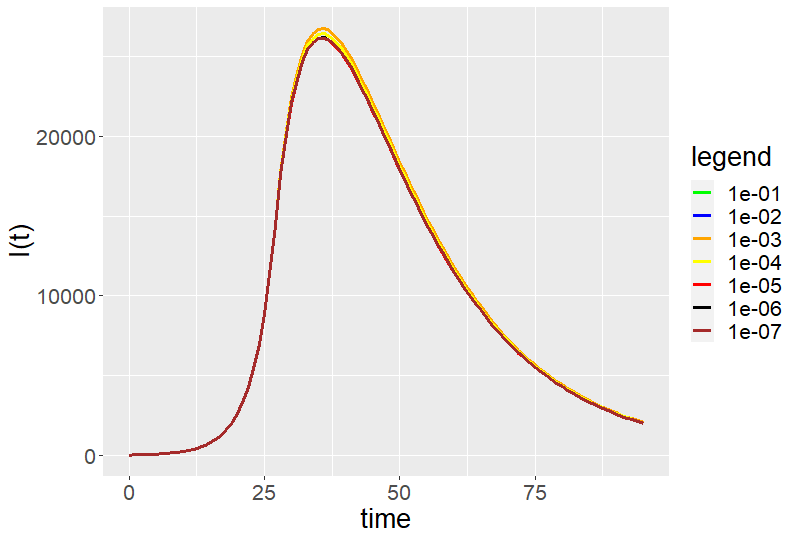
\includegraphics[width=0.7\linewidth]{./figures/tolerance_time_rk45_no_event_R}
	\caption{Time Discontinuity tolerance study on R's version of dopri5 without discontinuity handling}
	\label{fig:tolerance_time_rk45_no_event_R}
\end{figure}

\begin{figure}[h]
	\centering
	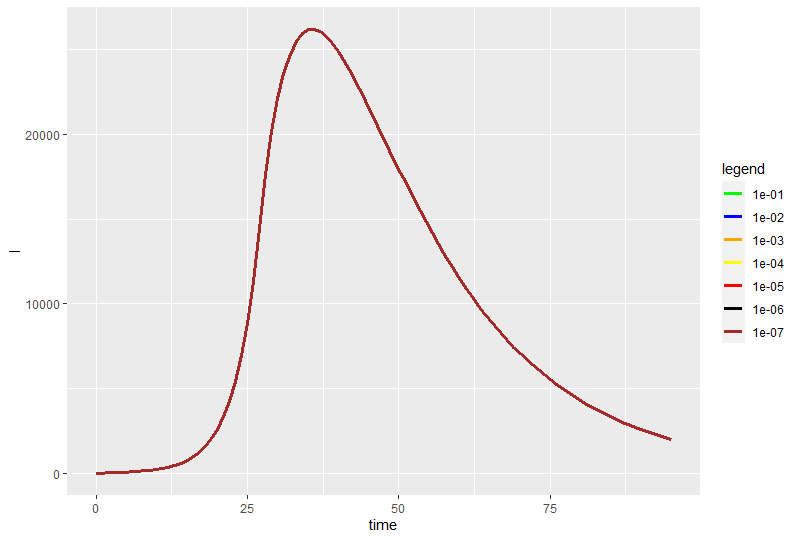
\includegraphics[width=0.7\linewidth]{./figures/tolerance_time_rk45_with_event_R}
	\caption{Time Discontinuity tolerance study on R's version of dopri5 with discontinuity handling}
	\label{fig:tolerance_time_rk45_with_event_R}
\end{figure}

From Figures $\ref{fig:tolerance_time_rk45_no_event_R}$ and $\ref{fig:tolerance_time_rk45_with_event_R}$, the addition of discontinuity handling lets us use a smaller tolerance and still get the required answer. Without discontinuity handling, we had to use $10^{-4}$ for both the absolute and relative tolerance but without, we seem to be able to use $10^{-1}$. 

However as we will see in the Python's version of DOPRI5, the results from $\ref{fig:tolerance_time_rk45_no_event_R}$ and $\ref{fig:tolerance_time_rk45_with_event_R}$ are suspicious and stem from the fact that R is not using interpolation to produce the results. It is using an old method that depends on the selected output points which affects efficiency and accuracy.


\begin{table}[h]
\caption {R dopri5 Time Discontinuity tolerance study} \label{tab:tolerance_time_discontinuity_rk45_R} 
\begin{center}
\begin{tabular}{ c c c c c }
tolerance & nfev & nsteps & event nfev & event nsteps \\ 
1e-01 & 572 &  95 & 574 &  95 \\
1e-02 & 572 &  95 & 574 &  95 \\
1e-03 & 572 &  95 & 574 &  95 \\
1e-04 & 612 & 101 & 574 &  95 \\
1e-05 & 692 & 113 & 587 &  97 \\
1e-06 & 735 & 120 & 599 &  99 \\
1e-07 & 926 & 150 & 702 & 116 \\
\end{tabular}
\end{center}
\end{table}

Table $\ref{tab:tolerance_time_discontinuity_rk45_R}$ also confirms our suspicions as at coarser tolerances, 1e-01 to 1e-3, the number of function evaluations does not change at all. This indicates that something else, not the tolerance nor the discontinuity, is the limiting factor for the number of function evaluations and that this other factor requires 572 or 574 function evaluations.

We suspect that R's DOPRI5 version is not using interpolation or some other dense output technique to produce its solutions and that it is integrating using the sampling points. That is, even though DOPRI5 is an algorithm that does not have a fixed step-size, R is forcing it to step from one output point to the other output point and thus our set of sampling points is a limiting factor. We then do the following experiment where we give R a smaller set of output points with the points are further away from each other and see what happens.

\begin{figure}[h]
	\centering
	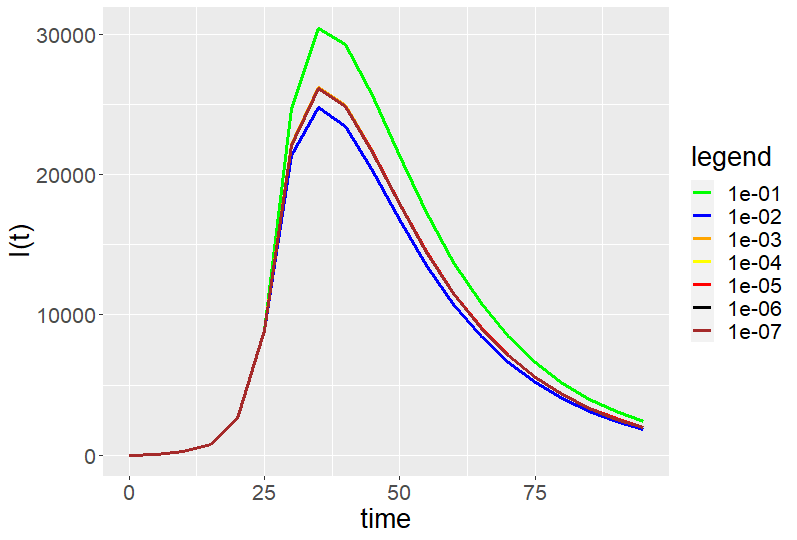
\includegraphics[width=0.7\linewidth]{./figures/tolerance_time_rk45_further_no_event_R}
	\caption{Time Discontinuity tolerance study on R's version of dopri5 without discontinuity handling and output points more space out}
	\label{fig:tolerance_time_rk45_further_no_event_R}
\end{figure}

\begin{figure}[h]
	\centering
	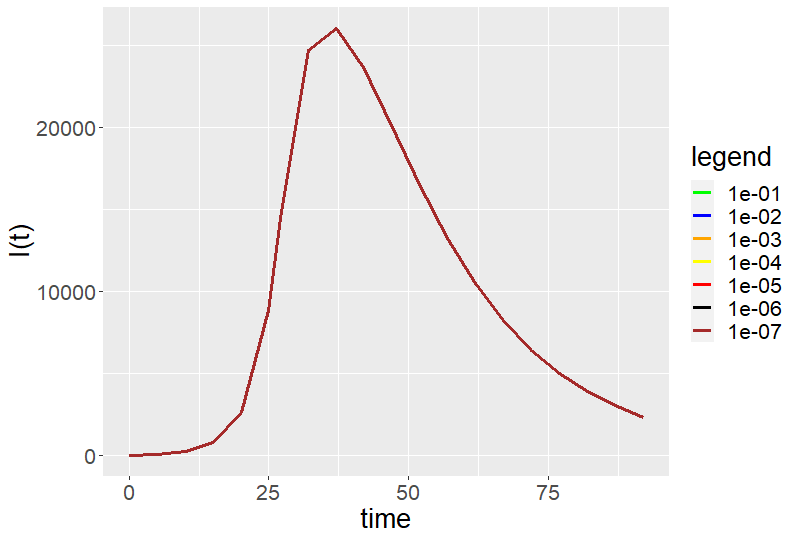
\includegraphics[width=0.7\linewidth]{./figures/tolerance_time_rk45_further_with_event_R}
	\caption{Time Discontinuity tolerance study on R's version of dopri5 with discontinuity handling and output points more space out}
	\label{fig:tolerance_time_rk45_further_with_event_R}
\end{figure}

From Figures $\ref{fig:tolerance_time_rk45_further_no_event_R}$ and $\ref{fig:tolerance_time_rk45_further_with_event_R}$, we can now see a more drastic change in the solution from the codes the output points further spaced out. Also, see table $\ref{tab:tolerance_time_discontinuity_rk45_further_R}$ where we will see the number of function evaluations actually change.

Using these two figures, we also see that discontinuity handling is allowing us to use coarser tolerances. We are able to use even $10^{-1}$ with discontinuity handling while getting an accurate result whereas without it, we need to use $10^{-3}$ and sharper tolerances to get the required answer.

\begin{table}[h]
\caption {R DOPRI5 Time Discontinuity tolerance study with spaced out points} \label{tab:tolerance_time_discontinuity_rk45_further_R} 
\begin{center}
\begin{tabular}{ c c c c c }
tolerance & nfev & nsteps & event nfev & event nsteps \\ 
1e-01 & 116 &  19 & 112 & 18 \\
1e-02 & 142 &  23 & 125 & 20 \\
1e-03 & 168 &  27 & 131 & 21 \\
1e-04 & 246 &  39 & 162 & 26 \\
1e-05 & 352 &  56 & 235 & 38 \\
1e-06 & 614 &  97 & 349 & 57 \\
1e-07 & 796 & 128 & 542 & 89 \\
\end{tabular}
\end{center}
\end{table}

Our analysis of Table $\ref{tab:tolerance_time_discontinuity_rk45_further_R}$ begins by noting that the set of output points is not longer a limiting factor. We can see the number of function evaluation change with the tolerance now and this indicates that the tolerance is affecting the step-size.This confirms our suspicions that R's implementation of DOPRI5 is not using a dense output mode or some form of interpolation. Instead it makes a steps to and stops at every required output points. This is the old way of giving function values at specified output points. 

Regarding the accuracy of the solver as we coarsen the tolerance we can see from Figures $\ref{fig:tolerance_time_rk45_further_no_event_R}$ and $\ref{fig:tolerance_time_rk45_further_with_event_R}$ that even at $10^{-1}$, the code with the discontinuity handling is still able to produce accurate solutions whereas it requires $10^{03}$ for the one without the discontinuity handling.

The new table, Table $\ref{tab:tolerance_time_discontinuity_rk45_further_R}$, does offer some more insights. Again we can see that at coarser tolerances, the decrease in the number of function evaluations is small but as the tolerance is sharpened, the number of function evaluations decreases significantly. The relatively similar number of function evaluations at the coarser tolerances does not excuse that the code without discontinuity handling is not getting the correct answer. 

\subparagraph{Time discontinuity tolerance study on Python's version of DOPRI5}
In this section, we run Python's version of DOPRI5, which is aliased under 'RK45' from the $solver\_ivp()$ function, with multiple tolerances with and without discontinuity handling. We will set both the relative and absolute tolerances to particular values and see how coarse we can keep the tolerance while still having correct results. We also look at efficiency data to see the decreases in the number of function evaluations.

\begin{figure}[h]
	\centering
	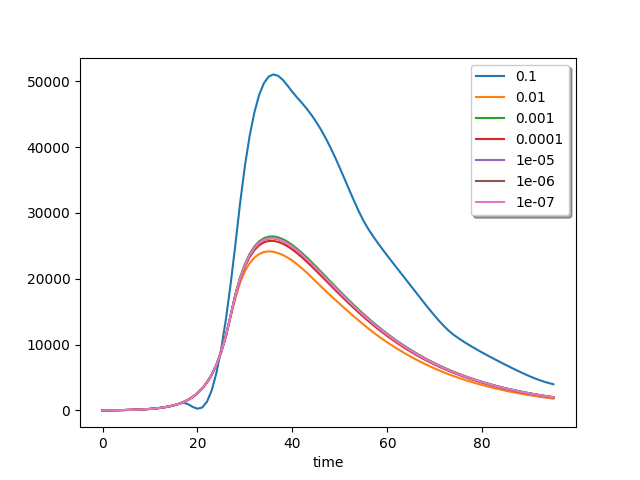
\includegraphics[width=0.7\linewidth]{./figures/tolerance_time_rk45_no_event_py}
	\caption{Time Discontinuity tolerance study on Python's version of dopri5 without discontinuity handling}
	\label{fig:tolerance_time_rk45_no_event_py}
\end{figure}

\begin{figure}[h]
	\centering
	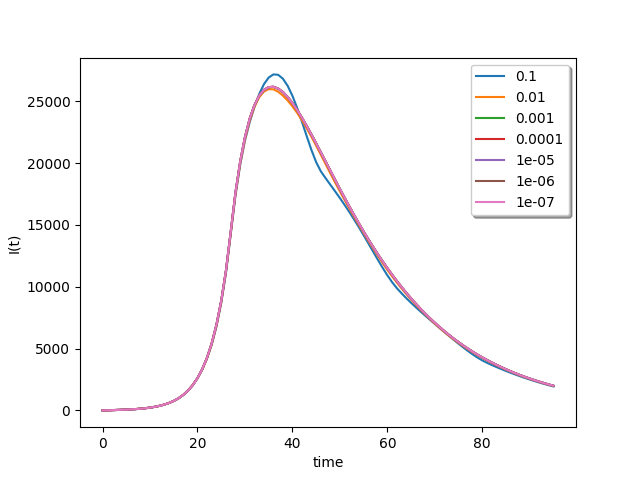
\includegraphics[width=0.7\linewidth]{./figures/tolerance_time_rk45_with_event_py}
	\caption{Time Discontinuity tolerance study on Python's version of dopri5 with discontinuity handling}
	\label{fig:tolerance_time_rk45_with_event_py}
\end{figure}

From Figures $\ref{fig:tolerance_time_rk45_with_event_py}$ and $\ref{fig:tolerance_time_rk45_no_event_py}$, we can see clearer differences at the different tolerance values. This is in contrast with the first tolerance study on R's DOPRI5. From studying Python's $solve\_ivp$ interface and source code, we note that Python is definitely using dense output/interpolation. This  concludes the discussion on R's DOPRI5 and we can explain R's DOPRI4 performance entirely because it does not use interpolation by default but instead stops at every output point.

We then compare Python's DOPRI5 with and without discontinuity handling. We can see that the use of discontinuity handling allowed us to use coarser tolerances in Python while keeping accurate results. We see that we need $10^{-5}$ and sharper to get the correct solutions without discontinuity handling in Python while $10^{-2}$ was enough with discontinuity handling. We will also see in Table $\ref{tab:tolerance_time_discontinuity_rk45_py}$ that the discontinuity handling code is much more efficient as well.


\begin{table}[h]
\caption {Python DOPRI5 Time Discontinuity tolerance study} \label{tab:tolerance_time_discontinuity_rk45_py} 
\begin{center}
\begin{tabular}{ c c c }
tolerance & nfev & event nfev \\ 
0.1   & 68.0  & 70.0  \\
0.01  & 86.0  & 88.0  \\
0.001 & 146.0 & 124.0 \\
0.0001& 224.0 & 172.0 \\
1e-05 & 326.0 & 250.0 \\
1e-06 & 488.0 & 370.0 \\
1e-07 & 752.0 & 568.0 \\
\end{tabular}
\end{center}
\end{table}

From Table $\ref{tab:tolerance_time_discontinuity_rk45_py}$, we see that at coarser tolerances, the number of function evaluations is lower in Python without the discontinuity handling than wit. But we should also point out that in Python, DOPRI5 at coarse tolerances gives very erroneous results and these do not excuse the small gain in efficiency.

At sharper tolerance where we get accurate results both with and without discontinuity handling and thus a fair comparison can be done, we can see that the code with discontinuity handling performs much better. At $10^{-7}$, the drop in the number of function evaluations is very significant and would lead to much faster execution times whereas at $10^{-5}$ and sharper, the decrease in the number of function evaluations is 75 or more.

\subparagraph{Time discontinuity tolerance study on Scilab's version of RKF45}
In this Section we run Scilab's RKF45 aliased as 'rkf' in the $ode()$ function with different tolerances. We note that the default tolerance for Scilab's 'rkf' was not enough to solve the problem without discontinuity handling but using cold starts did solve the problem even with that default tolerance. 

By running 'rkf' at various tolerances, we will show that it can also come up with the correct solutions at sharper tolerances without a discontinuity. Thus the anomaly we saw in section $\ref{subsection:naive_time_problem}$ was entirely because the solver has a coarser default tolerance in Scilab than the other methods.

We will also see that using the discontinuity handling lets us use less function evaluations which, given a more complex problem, will be a significant improvement in computation times.

\begin{figure}[h]
	\centering
	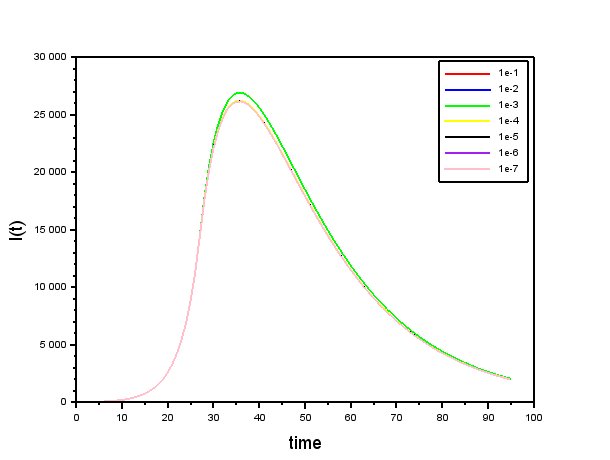
\includegraphics[width=0.7\linewidth]{./figures/tolerance_time_rk45_no_event_sci}
	\caption{Time Discontinuity tolerance study on Scilab's RKF45 without discontinuity handling}
	\label{fig:tolerance_time_rk45_no_event_sci}
\end{figure}

\begin{figure}[h]
	\centering
	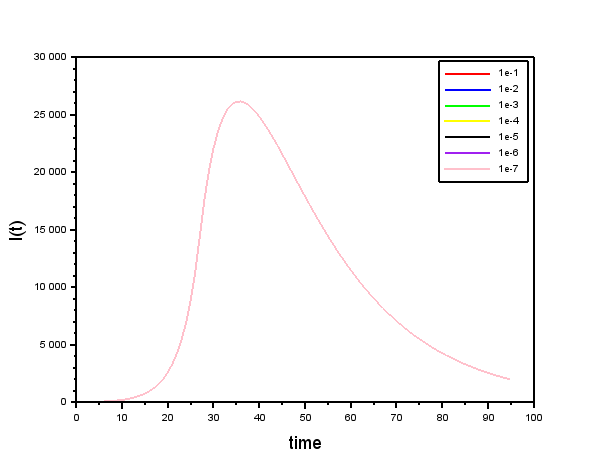
\includegraphics[width=0.7\linewidth]{./figures/tolerance_time_rk45_with_event_sci}
	\caption{Time Discontinuity tolerance study on Scilab's RKF45 with discontinuity handling}
	\label{fig:tolerance_time_rk45_with_event_sci}
\end{figure}

We see from Figure $\ref{fig:tolerance_time_rk45_no_event_sci}$ that $10^{-4}$ for both the absolute and the relative tolerance give accurate answers and that anything coarser does not work. We then remember that the relative tolerance defaults to $10^{-3}$ and the absolute tolerance defaults to $10^{-4}$ for 'rkf' which is slightly coarser than what was needed to get this correct solution.

Figure $\ref{fig:tolerance_time_rk45_with_event_sci}$ is also interesting as it seems to indicate that a $10^{-1}$ is enough to get the correct solution with discontinuity handling. This is also surprising but is consistent with our observations in R and Python's Runge-Kutta pairs.

\begin{table}[h]
\caption {Scilab RKF45 Time Discontinuity tolerance study} 
\label{tab:tolerance_time_discontinuity_rk45_scilab} 
\begin{center}
\begin{tabular}{ c c c }
tolerance & nfev  & event nfev \\ 
    0.1  & 577.  & 584. \\
    0.01  & 577. & 584. \\
    0.001  & 583. &  584. \\
    1e-4  & 641.  &  590. \\
    1e-5  & 674.  &  608. \\
    1e-6 &  847.  &  764. \\
    1e-7  & 924.  & 830.   \\
\end{tabular}
\end{center}
\end{table}

VI ===============================
IT SEEMS Scilab's rkf is NOT using interpolation
================================ VI

